%% Creator: Inkscape 0.91, www.inkscape.org
%% PDF/EPS/PS + LaTeX output extension by Johan Engelen, 2010
%% Accompanies image file 'Region_based.pdf' (pdf, eps, ps)
%%
%% To include the image in your LaTeX document, write
%%   \input{<filename>.pdf_tex}
%%  instead of
%%   \includegraphics{<filename>.pdf}
%% To scale the image, write
%%   \def\svgwidth{<desired width>}
%%   \input{<filename>.pdf_tex}
%%  instead of
%%   \includegraphics[width=<desired width>]{<filename>.pdf}
%%
%% Images with a different path to the parent latex file can
%% be accessed with the `import' package (which may need to be
%% installed) using
%%   \usepackage{import}
%% in the preamble, and then including the image with
%%   \import{<path to file>}{<filename>.pdf_tex}
%% Alternatively, one can specify
%%   \graphicspath{{<path to file>/}}
%%
%% For more information, please see info/svg-inkscape on CTAN:
%%   http://tug.ctan.org/tex-archive/info/svg-inkscape
%%
\begingroup%
  \makeatletter%
  \providecommand\color[2][]{%
    \errmessage{(Inkscape) Color is used for the text in Inkscape, but the package 'color.sty' is not loaded}%
    \renewcommand\color[2][]{}%
  }%
  \providecommand\transparent[1]{%
    \errmessage{(Inkscape) Transparency is used (non-zero) for the text in Inkscape, but the package 'transparent.sty' is not loaded}%
    \renewcommand\transparent[1]{}%
  }%
  \providecommand\rotatebox[2]{#2}%
  \ifx\svgwidth\undefined%
    \setlength{\unitlength}{304bp}%
    \ifx\svgscale\undefined%
      \relax%
    \else%
      \setlength{\unitlength}{\unitlength * \real{\svgscale}}%
    \fi%
  \else%
    \setlength{\unitlength}{\svgwidth}%
  \fi%
  \global\let\svgwidth\undefined%
  \global\let\svgscale\undefined%
  \makeatother%
  \begin{picture}(1,0.26315789)%
    \put(0.19736916,0.22368506){\color[rgb]{0,0,0}\makebox(0,0)[b]{\smash{\footnotesize $x_1$}}}%
    \put(0.28947443,0.17105364){\color[rgb]{0,0,0}\makebox(0,0)[lb]{\smash{\footnotesize $x_2$}}}%
    \put(0.30263232,0.07894805){\color[rgb]{0,0,0}\makebox(0,0)[lb]{\smash{\footnotesize $x_3$}}}%
    \put(0.13157969,0.02631664){\color[rgb]{0,0,0}\makebox(0,0)[b]{\smash{\footnotesize $x_4$}}}%
    \put(0.1052639,0.15789574){\color[rgb]{0,0,0}\makebox(0,0)[rb]{\smash{\footnotesize $x_5$}}}%
    \put(0.93421229,0.15789574){\color[rgb]{0,0,0}\makebox(0,0)[lb]{\smash{\footnotesize $\tilde{x}_1$}}}%
    \put(0.93421229,0.06842158){\color[rgb]{0,0,0}\makebox(0,0)[lb]{\smash{\footnotesize $\tilde{x}_2$}}}%
    \put(0.85055767,0.05170405){\color[rgb]{0,0,0}\makebox(0,0)[rb]{\smash{\footnotesize $\tilde{x}_3$}}}%
    \put(0.76842282,0.13157995){\color[rgb]{0,0,0}\makebox(0,0)[rb]{\smash{\footnotesize $\tilde{x}_4$}}}%
    \put(0.87492515,0.19524203){\color[rgb]{0,0,0}\makebox(0,0)[lb]{\smash{\footnotesize $\tilde{x}_5$}}}%
    \put(0.52631619,0.13157915){\color[rgb]{0,0,0}\makebox(0,0)[b]{\smash{$\overset{\textrm{korespondence}}{\Longleftrightarrow}$}}}%
    \put(0,0){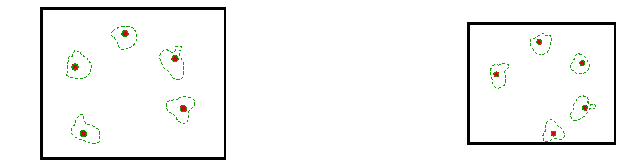
\includegraphics[width=\unitlength,page=1]{Region_based.pdf}}%
  \end{picture}%
\endgroup%
